\chapter{Résumé en Français}
\label{app:fr_long}

Nous fournissons ici un résumé en langue française des travaux présentés dans ce manuscrit de thèse.

\textbf{Résumé :}
%%%%%%%%%%%%%%%%%%%%%% ATTENTION ! SI MODIFICATION => MODIF SUR ADUM AUSSI !!!
L’arrivée des robots dans notre vie quotidienne fait émerger le besoin pour ces systèmes d’avoir accès à une représentation poussée des connaissances et des capacités de raisonnements associées. Ainsi, les robots doivent pouvoir comprendre les éléments qui composent l’environnement dans lequel ils évoluent. De plus, la présence d’humains dans ces environnements et donc la nécessité d’interagir avec eux amènent des exigences supplémentaires. Ainsi, les connaissances ne sont plus utilisées par le robot dans le seul but d’agir physiquement sur son environnement mais aussi dans un but de communication et de partage d’information avec les humains. La connaissance ne doit plus être uniquement compréhensible par le robot lui-même mais doit aussi pouvoir être exprimée.

Dans la première partie de cette thèse, nous présentons Ontologenius. C’est un logiciel permettant de maintenir des bases de connaissances sous forme d’ontologie, de raisonner dessus et de les gérer dynamiquement. Nous commençons par expliquer en quoi ce logiciel est adapté aux applications d’interaction humain-robot (HRI), notamment avec la possibilité de représenter la base de connaissances du robot mais aussi une estimation des bases de connaissances des partenaires humains ce qui permet d’implémenter les mécanismes de théorie de l’esprit. Nous poursuivons avec une présentation de ses interfaces. Cette partie se termine par une analyse des performances du système ainsi développé.

Dans une seconde partie, cette thèse présente notre contribution à deux problèmes d’exploration des connaissances: l’un ayant trait au référencement spatial et l’autre à l’utilisation de connaissances sémantiques. Nous commençons par une tâche de description d’itinéraires pour laquelle nous proposons une ontologie permettant de décrire la topologie d’environnements intérieurs et deux algorithmes de recherche d’itinéraires. Nous poursuivons avec une tâche de génération d’expression de référence. Cette tâche vise à sélectionner l’ensemble optimal d’informations à communiquer afin de permettre à un auditeur d’identifier l’entité référencée dans un contexte donné. Ce dernier algorithme est ensuite affiné pour y ajouter les informations sur les activités passées provenant d’une action conjointe entre un robot et un humain, afin de générer des expressions encore plus pertinentes. Il est également intégré à un planificateur de tâches symbolique pour estimer la faisabilité et le coût des futures communications.

Cette thèse se termine par la présentation de deux architectures cognitives, la première utilisant notre contribution concernant la description d’itinéraire et la seconde utilisant nos contributions autour de la Génération d’Expression de Référence. Les deux utilisent Ontologenius pour gérer la base de connaissances sémantique. À travers ces deux architectures, nous présentons comment nos travaux ont amené la base de connaissances a progressivement prendre un rôle central, fournissant des connaissances à tous les composants du système. 

\section*{Introduction}

Dans cette thèse, nous présentons plusieurs contributions autour de l'utilisation d'ontologie comme moyen de représenter les connaissances pour le robot ainsi que pour représenter une estimation des connaissances des partenaires du robot. Une ontologie est un graphe de connaissances avec en plus une spécification formelle et explicite de la signification partagée des concepts qui y sont utilisés. En robotique, l'utilisation d'une telle représentation formelle et explicite permet une unification des connaissances au sein d'une architecture entière. La connaissance n'est plus omniprésente parmi les composants, chacun possédant la partie dont il a besoin sans accord. Avec une ontologie, la connaissance devient une ressource partagée. Cette notion de connaissance partagée est également importante lorsqu'on parle de systèmes multi-robots. L'utilisation d'une ontologie permet à tous les robots de communiquer en utilisant le même vocabulaire. Par conséquent, il peut faciliter leur interaction, même s'ils ne reposent pas sur la même architecture.

En étendant les applications multi-robots, nous atteignons les applications multi-agents et par conséquent les applications pour l'interaction homme robot. La connaissance qu'une ontologie représente est la connaissance de la façon dont nous, en tant qu'êtres humains, nous percevons notre environnement et comment nous l'interprétons. Certes une ontologie est compréhensible par la machine mais surtout, à la base, compréhensible par l'homme, à la différence des réseaux de neurones par exemple. Grâce à toutes ces caractéristiques et parce qu'elle vient de la connaissance humaine, l'ontologie peut convenir pour représenter une estimation de la connaissance humaine pour un robot. De plus, en essayant de l'aligner sur le savoir humain, de la même manière que plusieurs robots peuvent utiliser le vocabulaire qu'une ontologie contient pour communiquer, un robot pourrait l'utiliser pour communiquer avec un humain, que ce soit pour interpréter un acte de communication ou pour en produire un. 

\section*{Ontologenius : une mémoire sémantique pour l'interaction Homme-Robot}

Dans ce chapitre, nous présentons Ontologenius, un logiciel open source et léger pour maintenir un graphe de connaissances à l'aide d'une ontologie. Ce logiciel avait été développé pour des applications d'Interaction Homme-Robot avec la possibilité de maintenir plusieurs bases de connaissances à la fois, l'une représentant les connaissances du robot et les autres étant l'estimation des connaissances des partenaires du robot. De plus, concernant la gestion de plusieurs instances à la fois, Ontologenious est livré avec une fonctionnalité de copie profonde pour récupérer l'état d'une base de connaissances à un moment donné, puis pour la modifier librement. Pour représenter plusieurs états de connaissance d'un même agent et éviter la création de trop d'instances qui pourraient ralentir le CPU, avec Ontologenius nous avons proposé une sorte de système de versionnage, gardant une trace des changements. Concernant la récupération de connaissances, avec Ontologenius nous avons choisis de fournir un ensemble de requêtes précises travaillant au niveau sémantique mais permettant l'exploration de la structure de la connaissance plutôt que simplement les relations entre entités.

\subsection*{Conception et fonctionnalités}

Dans cette section, nous expliquons d'abord notre choix d'utiliser l'ontologie comme moyen de représentation des connaissances, tant du point de vue de son expressivité que de son utilisation croissante en robotique. Ensuite, nous présentons les fonctionnalités souhaitées et le niveau d'expressivité que nous avons sélectionné pour ce logiciel.

\subsubsection*{Pourquoi une ontologie ?}

En psychologie cognitive, la mémoire sémantique fait référence à la connaissance encyclopédique des mots associée à leur signification. Après plusieurs études sur les temps de réponse des participants aux questions, certains auteurs ont proposé un modèle de cette mémoire sémantique comme étant un réseau sémantique~\cite{collins_1969_retrieval, collins_1970_does}. Avec ce modèle, ils posent l'hypothèse que les connaissances sont organisées de manière hiérarchique, respectant un principe d'inclusion entre les classes. Par exemple, une classe représentant le concept de chat hériterait d'une classe supérieure, représentant le concept d'animal. De plus, les instances de ces classes seraient liées aux autres par des propriétés, et de la même manière que pour les classes, une notion de hiérarchie sur les propriétés existerait. Une telle structure des connaissances chez l'homme permettrait une économie cognitive ainsi qu'un stockage efficace de ces connaissances. Même s'ils n'ont pas été les premiers à formaliser le principe d'un réseau sémantique, Collins et Quillian ont fourni des travaux et des implémentations informatiques de premier plan.

Comme indiqué dans~\cite{prasad_2020_knowledge}, un tel réseau sémantique, également appelé graphe sémantique ou graphe de connaissances, est aujourd'hui fréquemment utilisé comme représentation de connaissances dans les applications robotiques pour représenter entre autres :

\begin{itemize}
   \item les catégories d'entités à différents niveaux d'abstraction~\cite{balint_2018_variations}, par ex. une poignée est un objet physique
   \item les caractéristiques des entités~\cite{tenorth_2017_representations}, par ex. un réfrigérateur a une poignée
   \item la fonction ou le but des entités~\cite{paulius_2019_functional}, par ex. la poignée du réfrigérateur permet d'ouvrir le réfrigérateur
   \item l'emplacement d'une entité par rapport à une autre (c'est-à-dire des relations spatiales)~\cite{singh_2020_fuzzy}, par ex. la bouteille de lait est au frigo
\end{itemize}

C'est sur la base de ces connaissances que nous pouvons ensuite créer des programmes pour fournir des capacités cognitives aux robots. Voici un point important, cette connaissance doit supporter les composants de l'architecture mais n'en fait pas forcément partie. C'est ce qu'on appelle le paradigme de la programmation robotique basée sur la connaissance~\cite{beetz_2012_cognition}, où la connaissance est séparée du programme. Il permet d'avoir plusieurs sous-systèmes d'une même architecture robotique, chacun apportant une capacité cognitive spécifique mais partageant tous les mêmes connaissances. Le choix de partager des connaissances communes entraîne des défis importants nécessitant d'abord de se mettre d'accord sur le contenu de la connaissance et ensuite de le fournir d'une manière compréhensible par la machine. Considérant l'utilisation d'un réseau sémantique comme représentation des connaissances, l'utilisation de l'ontologie est destinée à répondre à ces défis. 

La première définition d'une ontologie a été proposée par Guber dans~\cite{guber_1993_translational} comme suit : \textit{``une ontologie est une spécification explicite d'une conceptualisation''}. Plus tard, Borst~\cite{borst_1999_construction}, a introduit deux nouveaux concepts définissant une ontologie comme une \textit{``spécification formelle d'une conceptualisation partagée''}. Les nouveaux concepts sont les notions de « formel » et de « partagé ». En fusionnant ces deux définitions, Studer et al.~\cite{studer_1998_knowledge} sont parvenus à la définition : \textit{``Une ontologie est une spécification formelle et explicite d'une conceptualisation partagée''}. Avec cette dernière définition, on commence à voir qu'une ontologie peut être un outil puissant pour créer une base de connaissance commune à toute une architecture robotique et utilisée par des sous-systèmes fournissant des capacités cognitives spécifiques.

Même si toutes les définitions précédentes tendent à affiner ce qu'est une ontologie, elles reposent toutes sur la notion commune de conceptualisation pour laquelle aucune définition formelle n'est fournie. Une ancienne définition, présentée dans ~\cite{genesereth_1987_logical}, était :

\begin{quote} 
\centering 
\textit{
« Un corps de connaissances formellement représenté est basé sur une conceptualisation : les objets, concepts et autres entités qui sont supposés exister dans un domaine d'intérêt et les relations qui existent entre eux. Une conceptualisation est une vue abstraite et simplifiée du monde que nous souhaitons représenter dans un but précis. Chaque base de connaissances, système à base de connaissances ou agent de niveau de connaissance est engagé dans une certaine conceptualisation, explicitement ou implicitement.''}
\end{quote}

Cependant, comme l'explique Guarino dans~\cite{guarino_2009_ontology}, une telle définition d'une conceptualisation ne correspond ni à notre intuition ni à notre besoin d'une ontologie. En effet, nous ne voulons pas que la conceptualisation dépende de la situation actuelle. Il doit plutôt être ce qui est commun à toute situation, permettant de les représenter de manière uniforme. Comme expliqué dans ~\cite{guarino_1995_towards}, lorsque le monde est modifié, la conceptualisation doit rester la même. On s'intéresse donc au sens des concepts utilisés pour décrire un état du monde. Cependant, la définition finale d'une conceptualisation fournie par Guarino va difficilement dans ce sens malgré son objectif initial. Pour la simplicité du propos actuel, la conceptualisation devrait être le sens de tout concept permettant de représenter une situation ou un état du monde donné. Par conséquent, une ontologie pourrait être définie comme :

\begin{quote} 
\centering 
\textit{une spécification formelle et explicite du sens partagé de tout concept permettant de représenter une situation donnée.}
\end{quote}

En d'autres termes, une ontologie vise à contraindre l'interprétation d'un vocabulaire utilisé. C'est donc une théorie logique. Cependant, en regardant la littérature, nous remarquons que la définition d'une ontologie est encore aujourd'hui floue. En effet, même si elle représente le sens des concepts utilisables, nous souhaitons l'appliquer à la base de connaissance représentant un état du monde donné, même s'il évolue dans le temps. Là où un réseau sémantique représenterait cette instanciation, car la signification de ses arêtes pourrait être définie par l'utilisation d'une ontologie, dans cette thèse, nous utiliserons le terme ontologie pour désigner \textbf{un réseau sémantique possédant une restriction sur l'interprétation du vocabulaire utilisé}. Le but de cette thèse n'étant pas de modéliser ces règles de restriction mais plutôt de les utiliser, cela ne doit pas prêter à confusion. 

Considérant l'étude de l'ontologie en robotique, et plus généralement en informatique, on peut distinguer trois types d'apports :

\begin{itemize}
   \item création d'ontologie,
   \item stockage et inférence d'ontologies,
   \item framework utilisant une ontologie
\end{itemize}

La création d'ontologies se concentre sur la définition du vocabulaire et des règles. Les ontologies créées sont souvent divisées en quatre catégories : niveau supérieur, référence, domaine et application. Les ontologies de niveau supérieur définissent des concepts largement applicables, transversaux à plusieurs disciplines. Les plus utilisées sont DOLCE (Descriptive Ontology for Linguistic and Cognitive Engineering) \cite{masolo_2003_dolce}, Cyc \cite{lenat_1989_building}, ou SUMO (Suggested Upper Merged Ontology) ~\cite{niles_2001_towards}. Les ontologies de référence sont basées sur une ontologie supérieure et décrivent le vocabulaire d'une discipline, comme l'ingénierie ou la médecine. Par exemple, \cite{schlenoff_2015_ieee} couvre la robotique et l'automatisation, décrivant le robot d'un point de vue technique, avec ses capteurs, ses processus et sa pose. Les ontologies de domaine visent à affiner une discipline, en se concentrant sur un domaine plus restreint, comme l'ontologie SOMA~\cite{bessler_2020_foundations} se concentrant sur la représentation des activités. Enfin, les ontologies d'applications étendent les ontologies de domaine pour des applications précises. La conception de l'ontologie utilise des langages tels que RDF (Resources Description Framework), FOL (First Order Logic) ou OWL (Web Ontology Language). Chaque langage est livré avec des caractéristiques telles que la formalité ou la calculabilité.

À l'aide de ces ontologies, de nombreux frameworks ont été développés pour prendre en charge les processus de raisonnement de haut niveau dans les applications robotiques. Parmi elles, on trouve des ontologies utilisées pour la prise de décision, l'évaluation de situation, la planification ou le maintien de croyances. Un examen complet de ces capacités de raisonnement et des cadres correspondants est disponible dans ~\cite{olivares_2019_review}. Parmi les frameworks revus, les emblématiques sont KnowRob~\cite{tenorth_2013_knowrob}, ROSETTA~\cite{stenmark_2013_knowledge}, CARESSES~\cite{bruno_2017_caresses}, RoboBrain~\cite{saxena_2014_robobrain}, ou encore ORO~\cite{lemaignan_2010}.

Le dernier type de contribution, étant celui du chapitre actuel, est le stockage et l'inférence d'ontologies pour former une base de connaissance sur laquelle le framework peut s'appuyer pour effectuer un raisonnement de haut niveau. KnowRob utilise Prolog~\cite{wielemaker_2003_prolog} avec une bibliothèque pour gérer les triplets RDF. ROSETTA utilise un triple store Sésame~\cite{broekstra_2002_sesame}. ORO utilise le triple magasin Jena en plus du raisonneur Pellet~\cite{sirin_2007_pellet}. Enfin, RoboBrain utilise une base de données de graphiques personnalisée. Nous pouvons voir qu'aucune solution standard n'a émergé car elle dépend principalement des besoins de l'application en termes de capacité de requête, de prise en charge de l'expressivité ou de support technique et de compatibilité. Comme d'autres outils, nous pouvons trouver en C++ owlcpp~\cite{levin_2011_owl} basé sur Raptor et Fact++~\cite{tsarkov_2006_fact}, ou en Python RDFlib, OWLReady2 ou AllegroGraph. 

En résumé, une base de connaissances sous forme d'ontologie, peut être vue comme un graphe sémantique reposant sur une spécification formelle et explicite du sens partagé des concepts utilisés pour représenter une situation donnée. Afin d'être utilisée dans un cadre pour effectuer un raisonnement de haut niveau, l'ontologie doit être stockée pour exposer les connaissances qu'elle contient à d'autres composants. Aucune solution de stockage standard n'a vu le jour jusqu'à présent car elle dépend principalement des besoins de l'application. Par conséquent, dans la partie suivante de cette section, nous discutons de nos besoins en nous concentrant sur les applications d'interaction homme-robot et en nous inspirant des solutions existantes, nous définissons les fonctionnalités que nous souhaitons pour notre système de stockage.

\subsubsection*{Caractéristiques souhaitées}

\paragraph{Travailler en serveur :} L'architecture robotique que nous visons est composée de plusieurs modules, capables de communiquer. En plus de l'architecture, nous considérons un système de supervision, étant une sorte de ``chef d'orchestre'' qui appelle chaque composant en cas de besoin. Un problème commun avec une telle architecture est que chaque composant possède une partie des connaissances générales qui peuvent conduire à des incohérences. Par conséquent, la base de connaissances que nous voulons doit être un serveur, accessible par requête et mise à jour par n'importe quel composant. Il fournit ainsi une connaissance uniforme au sein de l'architecture. Pour créer un serveur, nous pourrions utiliser n'importe quel outil existant et lui attacher une couche de communication. C'est par exemple le cas d'ORO, qui fonctionne comme un serveur, basé sur le triple store Jena et fournissant une interface Telnet pour envoyer les requêtes et les mises à jour.

\paragraph{Supporter plusieurs instances :} Puisque nous ciblons l'application HRI, nous devons être en mesure de représenter une estimation des connaissances des partenaires humains. Là où certains pourraient utiliser une seule base de connaissances pour représenter les connaissances des robots ainsi que les connaissances des humains, nous voulons que notre logiciel prenne en charge la "distinction soi-autre". Il est présenté dans~\cite{pacherie_2012_phenomenology} comme le fait que ``pour des représentations partagées (...) intentions''. A notre connaissance, ORO est le seul logiciel proposant cette capacité. Cependant, il utilise un moyen simple de l'implémenter en exécutant plusieurs instances du même triple magasin, chacune attachée à un agent. Comme nous le verrons dans la suite, en application robotique une telle solution n'est pas suffisante. Pour l'utilisation de la planification des tâches, nous pourrions avoir besoin d'estimer un état futur d'une basse de connaissance. Pour implémenter cette fonctionnalité, il faut pouvoir capter l'état d'une basse de connaissance à un instant donné puis pouvoir le modifier sans impacter la basse de connaissance d'origine, qui est continuellement mise à jour par la perception. A la date de cette thèse, aucun outil à base d'ontologie n'offre cette possibilité.

\paragraph{Requête au niveau sémantique :} Comme expliqué dans~\cite{broekstra_2002_sesame}, pour interroger des graphes RDF, trois niveaux sont possibles. Considérant une ontologie écrite en XML, le niveau syntaxique interrogerait la structure XML. Par conséquent, il interrogerait un arbre plutôt qu'un graphe. Une requête serait ``donnez-moi les ressources imbriquées dans un élément \textit{Description} ayant l'attribut \textit{about} avec la valeur X''. Il est donc dépendant de la langue et nécessite de connaître les mots-clés utilisés. Le niveau structurel, tel qu'il est disponible dans ~\cite{lassila_1998_resource}, fournit une abstraction au langage. Il permet des requêtes du genre ``donnez-moi tous les éléments de type A'' quelle que soit la façon dont il est représenté dans le langage. Cependant, le niveau structurel ne regarde que les triplets explicites. Si B est un sous-type de A et que l'élément x est décrit comme étant de type B, demandant les éléments de type A, x ne sera pas renvoyé. Le dernier niveau de requête est le niveau sémantique qui ne se limite pas à des connaissances explicites. À ce niveau, en demandant les éléments de type A, x serait renvoyé car x est de type B et B est une spécification de A. Cela signifie que nous ne considérons pas un simple triple magasin essayant de faire correspondre des modèles. Pour supporter ce niveau de requête, deux solutions peuvent être utilisées : calculer la fermeture du graphe (ajouter A comme type de x et le stocker), ou l'inférer à la requête. Alors que la première solution supprime une partie de la sémantique en aplatissant la hiérarchie\footnote{On perd le fait que x est de type A car il est de type B.}, la seconde peut être chronophage pour les requêtes.

\paragraph{Requêtes spécifiques :} Nous visons à utiliser notre logiciel avec des algorithmes de solveur. Cela signifie que nous voulons fournir un accès fin aux connaissances stockées à haute fréquence. A la différence de Prolog ayant son propre algorithme de recherche, nous préférerions des requêtes de niveau inférieur telles que : ``quels sont les types directs de X ?'', ``quelles sont les propriétés inverses de Y ?'', ``quelles les propriétés relient C et D?'', ou ''E est-il dans le domaine d'application de F?'', et cela au niveau sémantique. Néanmoins, pour les requêtes rapides, nous devons faire attention au nombre d'inférences nécessaires au moment de la requête.

\paragraph{Reasoning at update :} Pour éviter trop d'inférences au moment de la requête, nous voulons que certaines inférences soient appliquées lors de la mise à jour. Bien que le calcul de la fermeture entière aplatirait la basse de connaissance, certaines relations peuvent encore être calculées lors de mises à jour comme celles provenant de relations inverses ou d'axiomes en chaîne.

\paragraph{Thread safe :} Puisque le logiciel doit fonctionner comme un serveur, nous voulons qu'il supporte plusieurs requêtes en parallèle mais qu'il soit sécurisé lors de la mise à jour.

\paragraph{Niveau d'expressivité :} Considérant le langage d'ontologie Web (OWL), il existe différents niveaux d'expressivité selon les besoins. Le plus expressif est OWL-full, cependant, il est dit qu'il n'est pas informatique, ce qui signifie que les inférences qu'il permet ne peuvent pas être résolues au moment de la requête. Ensuite, OWL-DL (Description Logic) prend en charge la hiérarchie des propriétés et des classes, la restriction de valeur d'énumération, les propriétés inverses ou la restriction de cardinalité. Enfin, OWL-lite est le moins expressif, ne supportant pas la restriction de cardinalité et la restriction de valeur. Même si OWL-DL conviendrait, dans une première version OWL-lite pourrait suffire. C'est pourtant l'expressivité minimale à soutenir dans son ensemble.

\paragraph{Raisonnement personnalisé :} À des fins de recherche, nous ne voulons pas nous limiter au raisonnement logique du premier ordre. Nous voulons pouvoir intégrer des processus de raisonnement applicatifs ayant un accès direct à la structure interne. Une telle fonctionnalité pourrait être fournie par le support de plugins par exemple. L'avantage des plugins est que n'importe qui peut ajouter des capacités de raisonnement sans modifier le noyau du logiciel ou posséder une version personnalisée.

Au vu de nos fonctionnalités souhaitées, du nombre d'outils disponibles mais plus maintenus ou sans documentation, et de notre besoin de pouvoir mettre en œuvre de nouvelles capacités en fonction de nos besoins de recherche évoluant dans le temps, nous choisissons de développer de nouveaux logiciels en partant de zéro. Le logiciel résultant est Ontologenius. Un tel choix est risqué car il sera difficile d'atteindre le niveau de logiciels beaucoup plus matures. En revanche, cela nous a permis au cours de cette thèse d'avoir la maîtrise de son fonctionnement interne et de pouvoir le faire évoluer facilement au cours des différents projets dans lesquels nous l'avons utilisé.

Ontologenius s'inscrit dans la continuité du logiciel ORO mais en proposant une gestion multi-instances plus poussée et un système de requêtes plus adapté à l'intégration dans des algorithmes. Jusqu'ici nous avons utilisé les termes de classe, propriétés, propriétés inverses, etc. Avant de commencer la présentation des fonctionnalités implémentées par Ontologenius, nous proposons d'abord une formalisation de ce qu'est une ontologie et une définition explicite des termes. Ce formalisme sera ensuite utilisé tout au long de ce document et donnera un aperçu de l'expressivité soutenue par Ontologenius à l'époque. 

\section*{Recherche d'un itinéraire avec des connaissances sémantiques}

Sur la base d'Ontologenius, nous présentons plusieurs contributions utilisant les connaissances stockées.

Nous avons tous déjà été sollicités, ou avons nous-mêmes demandé, notre chemin en ville, dans un centre commercial, ou plus simplement dans une maison. Lorsque nous fournissons de telles informations à une personne, nous effectuons ce que l'on appelle communément une tâche d'orientation. Même si cela peut sembler anodin pour nous, développer un robot capable de l'exécuter peut être un défi. Dans ce chapitre, nous choisissons de nous concentrer sur la sous-tâche consistant à générer la phrase d'explication. Cette sous-tâche s'appelle la description de l'itinéraire. Pour l'effectuer, nous avons d'abord besoin d'un ensemble de connaissances sur l'environnement dans lequel la personne guidée va marcher, comme les chemins, les intersections des chemins, ou les éléments qui les côtoient. Ensuite, nous avons besoin d'un ensemble de « bonnes pratiques » pour fournir un itinéraire assez facile à suivre et à retenir.

Dans le domaine de l'Interaction Homme-Robot (HRI), des robots guides ont été étudiés intensivement et déployés dans des centres commerciaux~\cite{okuno_2009_providing}, des musées~\cite{burgard_1999_museum, clodic_2006_rackham, siegwart_2003_robox}, ou des aéroports~\cite{triebel_2016_spencer}. D'un point de vue représentation des connaissances, on peut remarquer l'utilisation de représentations métriques~\cite{thrun_2007_simultaneous} ou topologiques~\cite{morales_2011_modeling} pour représenter l'environnement dans lequel le robot agit. Puisque nous nous concentrons sur la tâche de description d'itinéraire, nous considérons que le robot n'accompagne pas l'humain jusqu'à sa destination finale mais explique plutôt comment l'atteindre. Par conséquent, la représentation métrique ne sera pas considérée comme étant principalement utilisée à des fins de navigation~\cite{thrun_2007_simultaneous}. Pour effectuer plus spécifiquement une description d'itinéraire, la connaissance topologique n'est pas suffisante. En plus de la topologie de l'environnement, le robot a besoin de connaître les types des éléments composant l'environnement et leurs noms en langage naturel. Certaines contributions ont ainsi tenté de mélanger des représentations métriques ou topologiques avec des représentations sémantiques pour contenir ces connaissances supplémentaires~\cite {satake_2015_should, chrastil_2014_cognitive, zender_2008_conceptual}. Cependant, les mélanger peut créer un manque d'uniformité dans la représentation globale des connaissances. De cette façon, créer une représentation unique permettant à un robot de calculer des itinéraires et de les exprimer pourrait assurer l'uniformité des connaissances.

Même muni d'une représentation cohérente de son environnement, le robot doit trouver un itinéraire non pas pour lui-même mais pour l'humain guidé. Un robot accompagnant l'humain n'a qu'à déterminer un chemin, adapté à ses capacités et interprétable uniquement par lui-même. Fournissant un itinéraire à un humain, l'itinéraire doit être adapté aux capacités et aux connaissances humaines. Par exemple, dans un environnement extérieur, on ne donnera pas le même itinéraire pour un automobiliste ou un cycliste. Dans le cadre d'un centre commercial, nous ne donnerons pas de parcours avec escalier à une personne à mobilité réduite ou à une personne avec un caddie. Une fois calculé, le robot doit expliquer l'itinéraire. Là où les cartes interactives n'ont qu'à mettre en évidence un chemin, ici, le robot doit générer une phrase que l'humain pourra mémoriser. Bien sûr, le robot n'instruira pas un humain avec une phrase comme « marche de 30 mètres et tourne à -90 degrés ». Ce ne serait pas adapté. L'utilisation de l'orientation et de la référence aux éléments de l'environnement sera nécessaire à travers une phrase comme ``marcher jusqu'au fleuriste puis tourner à gauche''. Nous voulons donc que le robot génère des plans compréhensibles et exécutables par l'humain.

La première contribution de ce chapitre est une \textbf{représentation unifiée} d'un environnement intérieur utilisant une ontologie, pour inclure à la fois des connaissances topologiques et sémantiques. Ensuite, sur la base de cette représentation, nous proposons un premier algorithme pour \textbf{trouver un itinéraire approprié} à expliquer à un humain et un second algorithme pour \textbf{verbaliser un itinéraire} de manière appropriée. 

\section*{Génération d'expression de référence basée sur une ontologie}

Poursuivant sur l'exploitation des connaissances et plus précisément sur la communication spatiale, nous présentons maintenant une contribution autour de la tâche de génération d'expressions référentes.

Faire référence à une entité est l'une des tâches les plus courantes que nous effectuons chaque jour.`` Pouvez-vous m'apporter ma tasse ? C'est la noir à côté de l'évier''. ``Je ne me souviens pas du nom de l'homme avec la chemise rouge et les lunettes''. ``J'ai perdu mes clés, elles sont sur un porte-clés avec une peluche en forme de licorne''. Un tel type de communication, précis et efficace, est un aspect clé pour le succès d'une tâche collaborative. Néanmoins, dans des environnements complexes avec une grande variété d'objets, de lieux ou de personnes, faire référence à une entité spécifique peut devenir un véritable défi pour un robot. Elle doit tenir compte du contexte de la tâche supérieure, de la diversité des faits qui peuvent être extraits de la situation et qui dépendent des modalités de perception disponibles, et du terrain d'entente disponible entre le robot et son partenaire. 

\begin{figure}[ht!]
\centering
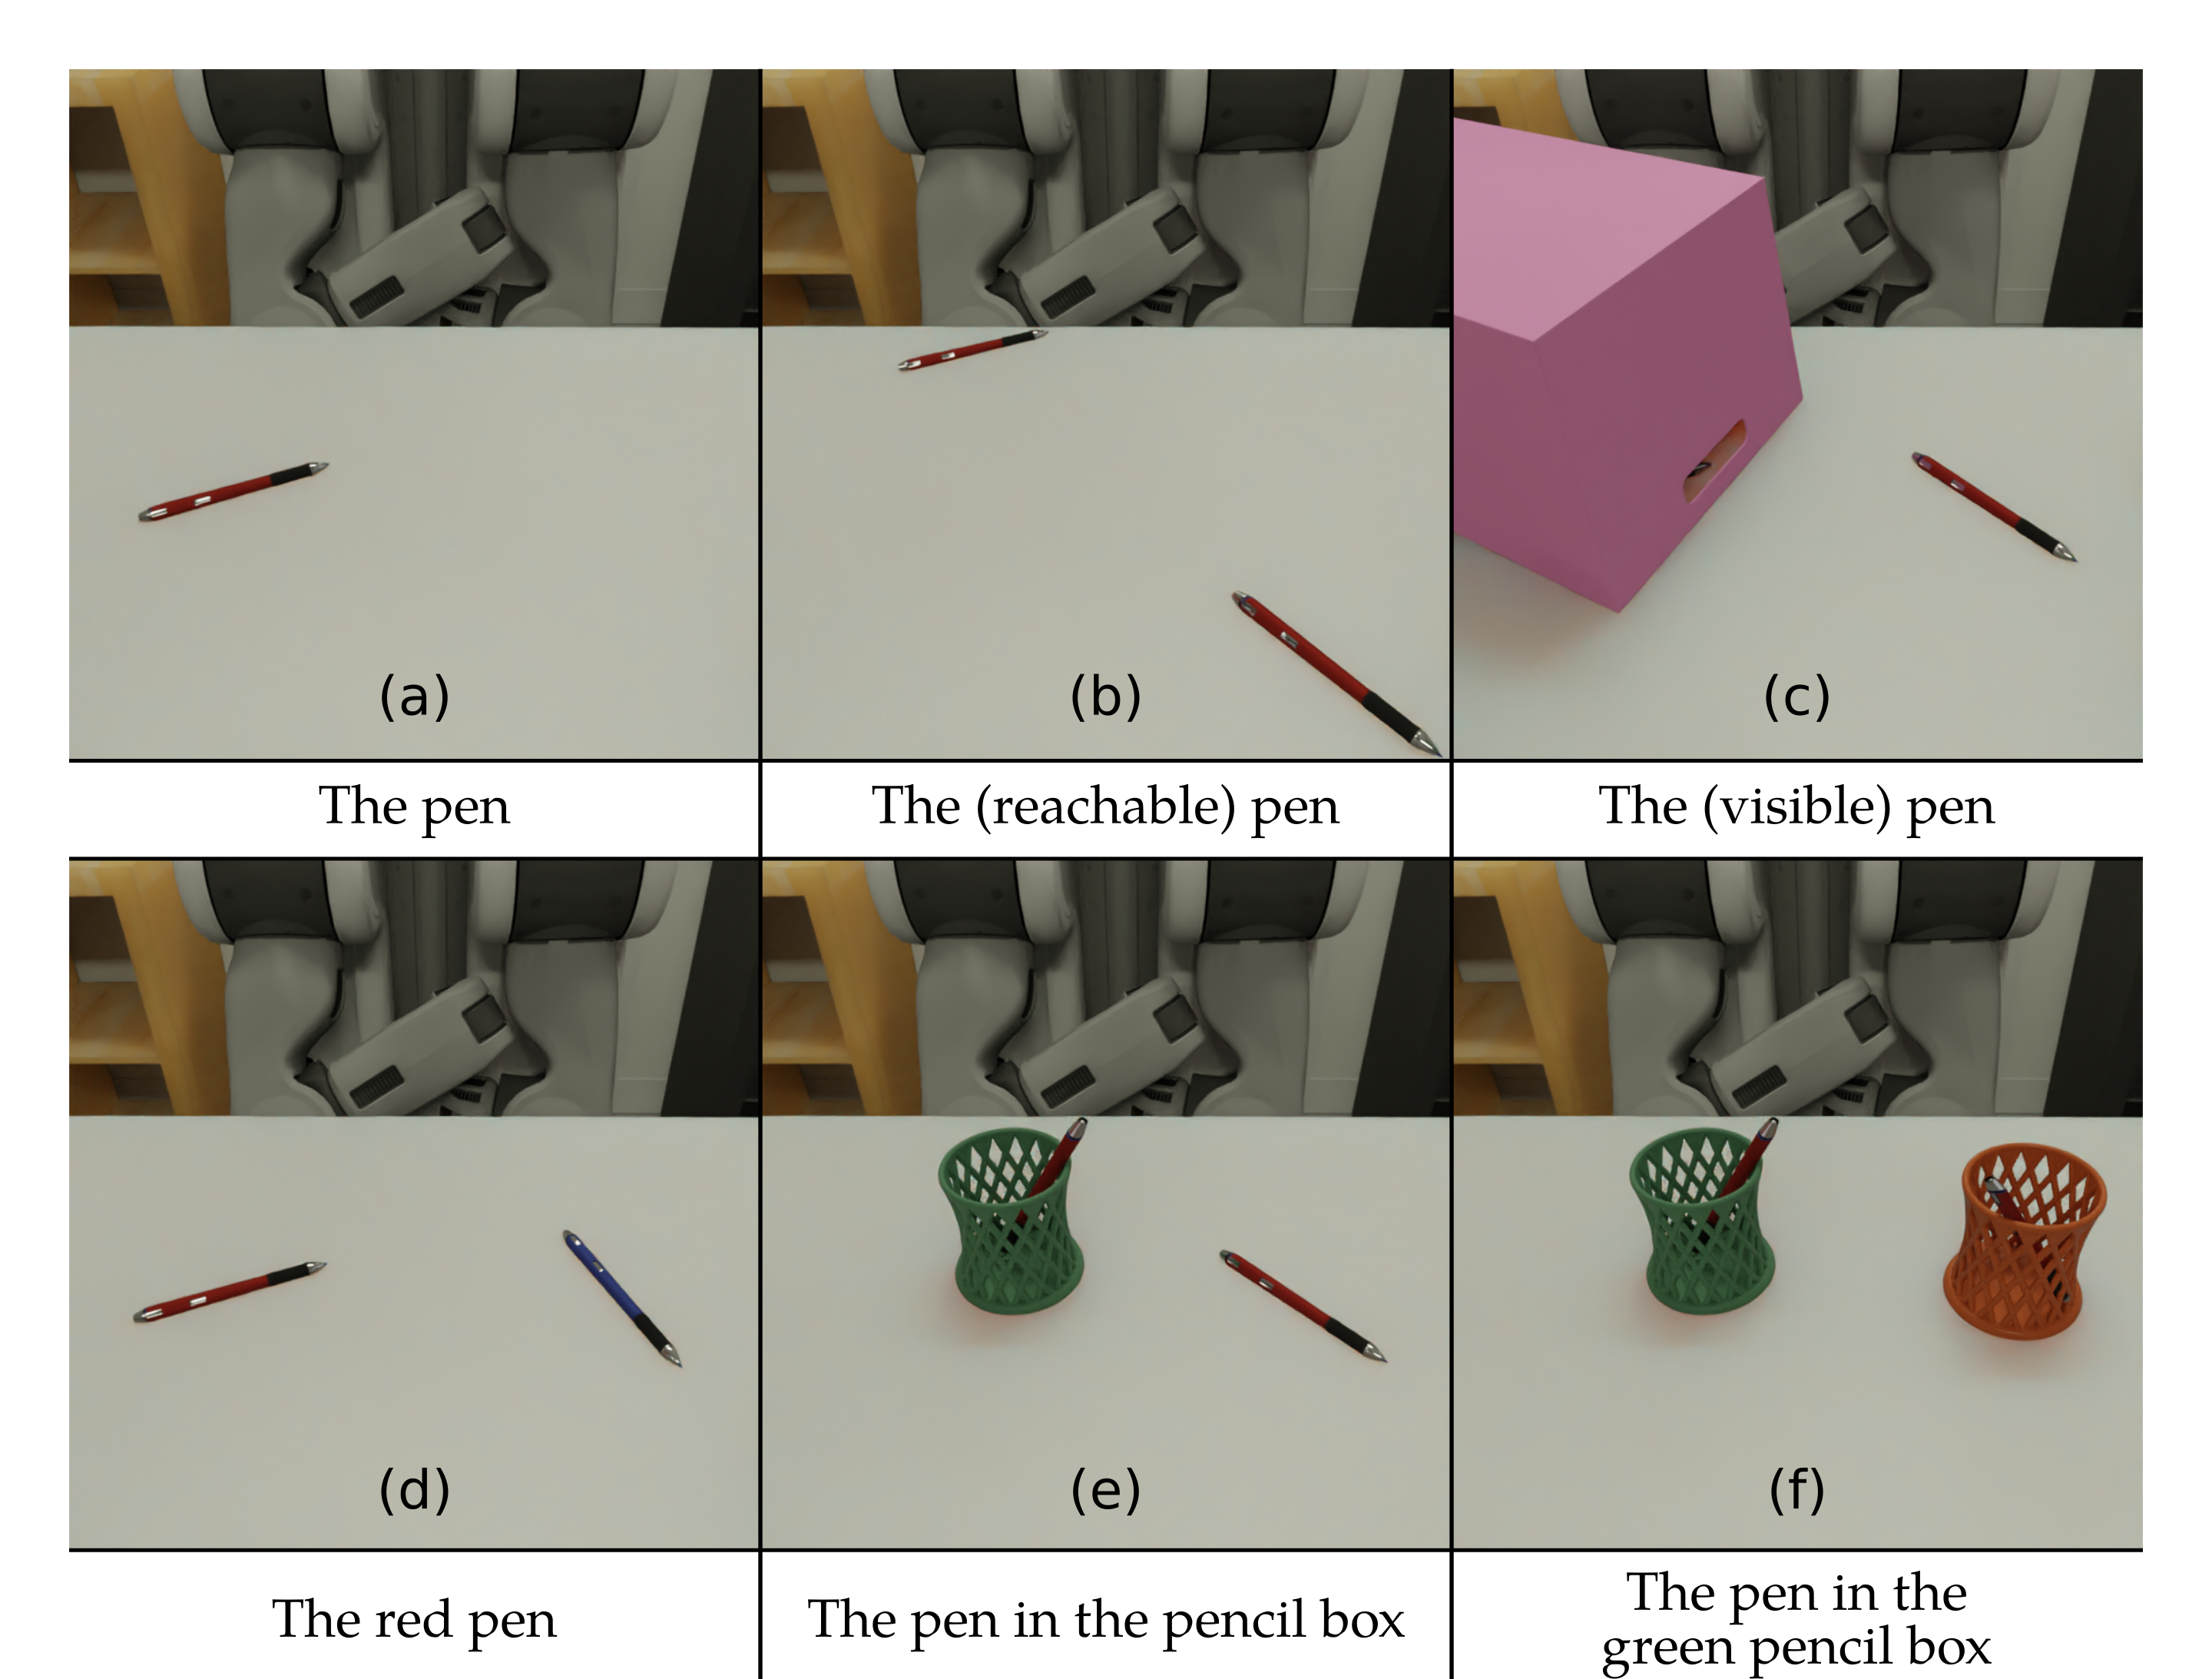
\includegraphics[scale=0.16]{figures/chapter4/intro.png}
\caption{\label{fig:annex_chap4_intro} Six situations vues du point de vue de l'auditeur, avec le robot placé de l'autre côté de la table. Se référer au même stylo implique différents mécanismes pour lever l'ambiguïté, dans chaque situation. La phrase en-dessous de chaque situation est une expression de référence possible pour désigner ledit stylo sans ambiguïté.}
\end{figure}

Considérez la situation où vous êtes autour d'une table avec votre robot collaboratif et le robot a besoin d'un stylo. La simple instruction \textit{``Donnez-moi le stylo''} peut entraîner plusieurs situations de complexités diverses. Dans le cas où il n'y a qu'un seul stylo (Fig.\ref{fig:annex_chap4_intro}a), s'y référer est évident. Considérons maintenant deux stylos sur la table. Si l'un est accessible par vous (l'humain) et l'autre ne l'est pas (Fig.\ref{fig:annex_chap4_intro}b), l'accessibilité peut être utilisée pour désigner le stylo. Si les deux stylos ne sont pas accessibles mais que l'un est visible pour vous et l'autre ne l'est pas (Fig.\ref{fig:annex_chap4_intro}c où un stylo est caché sous la boîte), la visibilité par prise de perspective peut être utilisée pour déterminer que le autre stylo ne conduit pas à l'ambiguïté. Maintenant, les deux stylos sont visibles et accessibles, mais l'un est bleu et l'autre est rouge (Fig.\ref{fig:annex_chap4_intro}d). L'ajout de la couleur du stylo résout l'ambiguïté. Si les deux stylos ont la même couleur mais que l'un est dans une boîte à crayons (Fig.\ref{fig:annex_chap4_intro}e), la relation avec la boîte à crayons résout l'ambiguïté. Si malheureusement, les deux sont dans une boîte à crayons mais l'un est vert et l'autre orange (Fig.\ref{fig:annex_chap4_intro}f), le rapport avec la boîte à crayons et la couleur de cette dernière lève l'ambiguïté. On pourrait continuer ainsi longtemps, en considérant qu'un est à votre gauche et un à votre droite, qu'il n'y a pas de stylo sur la table mais qu'il y en a un sur une étagère et ainsi de suite.

Jusqu'à présent, nous considérions que le robot connaissait les notions de stylo et de plumier ainsi que leurs noms en langage naturel pour en parler. Cependant, imaginez-vous voyager dans un autre pays et devoir parler anglais\footnote{Je m'excuse auprès des anglophones natifs qui ne profiteront pas pleinement de cet exemple.}, vous pouvez parfois manquer certains mots et donc en utiliser un plus générique à la place. Cependant, ce faisant, une nouvelle ambiguïté peut être levée car ce mot générique fait également référence à d'autres entités. Il en est de même pour notre robot s'il doit parler français et ne connaît pas la traduction du concept de la boîte à crayons. Il devra utiliser un terme plus générique, tel que « conteneur ». Cependant, ce terme plus générique pourrait également désigner d'autres entités, comme des boîtes.

En plus des noms de concepts, le robot doit faire attention aux relations qu'il utilise. Le poids ou la longueur exacte d'un objet ne serait pas utile car un humain ne peut pas facilement les évaluer. Au contraire, la couleur de l'objet semble être une propriété appropriée à utiliser, sauf si le robot partenaire est daltonien. Cela signifie que le robot doit utiliser des relations qu'il estime connues et facilement observables par son partenaire. Cela peut être fait en considérant la théorie de l'esprit et en effectuant la génération d'expression de référence sur la base de connaissances humaine estimée par le robot.

Cette tâche pour faire référence à une entité précise parmi d'autres est communément appelée la tâche \textbf{Referring Expression Generation (REG)}. Elle est souvent décomposée en deux sous-tâches : la \textbf{détermination du contenu} et la \textbf{réalisation linguistique}~\cite{krahmer_2012_computational}. La détermination de contenu vise à déterminer les relations à utiliser pour se référer à une entité tandis que la réalisation linguistique vise à choisir les mots à utiliser pour communiquer le contenu. La contribution de ce chapitre est centrée sur la détermination du contenu mais nous ne pouvons pas considérer ces deux sous-tâches comme entièrement indépendantes. Comme expliqué précédemment, si le robot ne connaît pas certains noms de concepts en langage naturel, la réalisation linguistique échouera dans le cas où la détermination du contenu les sélectionne. Une autre possibilité pour la réalisation linguistique serait de choisir un mot plus général mais il ne correspondrait pas au contenu déterminé. On pourrait imaginer une base de connaissances dédiée pour le REG avec uniquement des concepts utilisables en langage naturel, mais une telle solution n'est pas adaptée si l'on veut une base de connaissances unique pour tout le système robotique. De plus, il pourrait être difficile de maintenir cette base de connaissances dédiée pendant l'interaction, en plus d'autres car il s'agirait d'un dédoublement de connaissances.

La principale contribution présentée dans ce chapitre est un \textbf{algorithme basé sur une ontologie et indépendant du domaine pour la génération d'expressions référentes}. Il utilise une fonction de coût personnalisable estimant la charge cognitive nécessaire à un humain pour interpréter l'expression de référencement afin de produire \textbf{l'ensemble ``optimal'' d'assertions verbalisables} qui permet de se référer sans ambiguïté à une entité donnée.


Comme expliqué dans~\cite{reiter_2000_building}, il s'agit de ``comment produire une description d'une entité qui permet à l'auditeur d'identifier cette entité dans un contexte donné''. Alors que cette tâche est étudiée depuis des décennies, aucune des méthodes existantes n'a tenté d'utiliser une ontologie comme base de connaissances, travaillant la plupart du temps sur une base de connaissances dédiée à la tâche. De plus, parce que leur base de connaissances est dédiée à la tâche, elle n'est composée que de relations utilisable pour communiquer avec un humain. Cependant, compte tenu d'une base de connaissances partagée dans l'architecture, certaines connaissances peuvent avoir un usage purement technique pour le fonctionnement du robot. Plus important encore, aucun des travaux existants n'a vraiment pris en compte la notion de contexte. Leur seul but était de désigner une entité dans un état donné d'un environnement. Cependant, dans son utilisation pour de l'interaction homme-robot, la génération d'expression de référence n'est qu'une action d'une tâche plus large, dans laquelle un contexte existe, qu'il s'agit d'informations déjà connues sur l'entité à laquelle se référer ou d'une restriction implicite sur les entités concernées. Nous présentons ainsi un nouvel algorithme gérant toutes les problématiques précédemment évoquées et utilisant une ontologie comme base de connaissances. De plus, à travers des comparaisons avec d'autres algorithmes, nous montrons que notre contribution est, à ce jour, la plus efficace, résolvant de la plupart des problèmes en moins d'une milliseconde. Enfin, comme une preuve d'utilisabilité, l'algorithme a été intégré dans une architecture robotique avec une base de connaissances mise à jour en permanence par la perception. 

\section*{Estimation de la faisabilité et du coût de la communication lors de la planification des tâches}

Profitant de la haute performance de notre algorithme de génération d'expressions référentes, dans ce chapitre, nous proposons une méthode l'intégrant à un planificateur de tâches.

Il est bien établi qu'un aspect clé du succès des tâches collaboratives repose sur une communication claire et fluide ancrée dans le contexte de l'interaction. Centré sur la communication verbale, dans le domaine de recherche Traitement du langage naturel (TALN) et par extension dans le domaine de l'interaction humain-robot, il a été divisé en deux doubles problèmes~\cite{tellex_2020_robots}. D'une part, la compréhension du langage naturel (NLU) vise au robot à interpréter et à fonder les énoncés humains par rapport à la situation actuelle et à réagir en fonction de celle-ci~\cite{brawer_2018_situated}. D'un autre côté, la Natural Language Generation (NLG) vise au robot à produire du langage. Il peut s'agir soit de demander de l'aide~\cite{tellex_2014_asking}, d'aligner les connaissances~\cite{devin_2016_implemented}, soit d'expliquer sa décision à son partenaire~\cite{roncone_2017_transparent}.

Dans le chapitre précédent, nous avons introduit un algorithme capable de générer le contenu d'une expression référente. Une telle contribution relève donc du problème NLG. Considérer le REG comme une action pouvant être effectuée par le robot signifie que le robot pourrait planifier une telle communication en termes de \textbf{quand} et \textbf{quoi} pour communiquer. Alors que le ``quand'' est directement géré par le planificateur de tâches, le ``quoi'' en termes de contenu est fourni par le REG\footnote{Le REG ne détermine pas l'entité à laquelle se référer mais seulement comment elle sera référencée à. On pourrait dire que le « quoi » est choisi par une composante décisionnelle supérieure, tandis que le « comment » est déterminé par le REG. Pour correspondre à la définition habituelle, nous supposons cette simplification linguistique. }. Cependant, le REG ne fournit pas seulement le contenu mais est également en mesure d'indiquer si une telle communication est réalisable ou non et de donner des informations sur son coût. Dans le contexte du REG, la faisabilité de la communication est liée à la capacité à générer une expression référente sans ambiguïté alors que le coût dépend du nombre de relations à communiquer. Étant donné que l'algorithme REG fonctionne sur une base de connaissances représentant l'état actuel de l'environnement, le maintien d'une représentation comparable de l'environnement pour les états futurs de la tâche (comme cela se fait dans la planification symbolique des tâches) permettrait au robot d'estimer le \textbf {faisabilité} et le \textbf{coût} des actions de communication verbale tout au long d'une tâche.

Avec ces deux informations, à savoir le coût et la faisabilité, un planificateur de tâches pourrait comparer les communications verbales entre elles, comparer avec d'autres moyens de communication, minimiser la complexité globale de la communication et éviter certains échecs du plan. Cette approche pour estimer la communication lors de la planification des tâches peut être comparée à celle proposée dans ~\cite{lallement_2016_symbolic}. Dans ce dernier cas, les actions de mouvement ont été évaluées lors de la planification des tâches pour estimer leur faisabilité, leurs coûts et leurs effets indirects. Avec les deux approches, les plans symboliques peuvent être optimisés et peuvent être plus fiables pour prévenir les échecs d'exécution et donc le besoin de réparation. 

\begin{figure}[t!]
\centering
\includegraphics[width=\textwidth]{figures/chapter5/intro/intro.png}
\caption{\label{fig:annex_chap5_intro} Une tâche collaborative Homme-Robot avec trois zones colorées et trois tags RFID (situation a). Le robot doit expliquer à son partenaire humain de mettre le tag \textit{o1} dans la zone noire et le tag \textit{o2} dans la zone blanche, pour atteindre la situation d. Les identifiants des objets ne sont connus que du robot.
Si toutes les communications de la tâche ne sont pas planifiées à l'avance, une situation de blocage peut apparaître si le robot demande d'abord de déplacer la balise \textit{o1} avant \textit{o2} (situation b).}
\end{figure}

Pour mieux comprendre l'avantage de considérer la communication au niveau de la planification des tâches, considérons les situations de Figure~\ref{fig:annex_chap5_intro}. Le robot doit disposer des étiquettes RFID sur trois zones d'une table. Le robot peut les identifier avec leur identifiant unique mais étant trop petit, il ne peut pas les saisir. Au contraire, le partenaire humain ne peut pas les identifier de manière unique mais peut les saisir. Pour cet exemple, nous supposons également que le robot ne peut pas pointer vers les balises. Le robot doit donc communiquer les actions successives que l'humain devra effectuer pour passer de la configuration initiale (\ref{fig:annex_chap5_intro} a) à la configuration but (\ref{fig:annex_chap5_intro} d). Entre les deux configurations, seules les balises \textit{o1} et \textit{o2} doivent être déplacées. La balise \textit{o1} doit être déplacée de la zone rouge vers la zone noire et \textit{o2} de la zone noire vers la zone blanche. Alors que la balise \textit{o3} peut être référencée sans ambiguïté grâce à sa couleur, les deux autres ne le peuvent pas. Cependant, ils peuvent être référencés grâce à la zone dans laquelle ils se trouvent (par exemple \textit{``la balise est la zone rouge''}).

Si le contenu des communications n'est affiné qu'à l'exécution, deux solutions équivalentes peuvent être envisagées (\ref{fig:annex_chap5_intro} séquence a-b-d et a-c-d). A l'exécution, la première solution commence par demander à l'humain de déplacer \textit{o1} dans la zone noire résultant en l'instruction \textit{``prendre la balise qui est dans la zone rouge et la mettre dans la zone noire''} . Dans cette nouvelle situation où les deux balises rouges sont maintenant dans la zone noire (Figure~\ref{fig:annex_chap5_intro}b). Le robot n'a aucun moyen de désigner la balise \textit{o2} sans ambiguïté. Par conséquent, la tâche est bloquée\footnote{Le robot pourrait utiliser des relations spatiales comme la droite, la gauche ou le plus proche de moi. Cependant, la génération d'une telle expression de référence n'est pas une tâche facile et sa compréhension non plus. Même si la situation n'est pas vraiment bloquée, la communication requise peut être complexe. }. L'estimation de la faisabilité et du coût de la communication au cours du processus de planification aboutirait à la deuxième solution possible. Le robot demande d'abord de déplacer la balise \textit{o2} (Figure~\ref{fig:annex_chap5_intro} c) puis la balise \textit{o1} (Figure~\ref{fig:annex_chap5_intro} d). Si le robot avait pu pointer, l'impasse de la première solution peut être évitée avec une action de pointage et néanmoins, grâce à l'estimation des coûts de communication, la solution la moins chère peut être sélectionnée\footnote{Beaucoup d'autres solutions pourraient exister mais dépendent de la capacité robotique. Donner les deux instructions dans l'état initial avant l'acte humain résout aussi le problème par exemple. Néanmoins, si le robot ne peut pas comparer ces différentes solutions au regard de sa capacité actuelle, des situations non souhaitables peuvent encore apparaître.}.

La principale contribution présentée dans ce chapitre est une approche pour \textbf{estimer la faisabilité et le coût de la communication au niveau de la planification des tâches}. Cela implique un \textbf{lien fin entre un planificateur et une ontologie} pour estimer la communication ancrée dans l'état futur estimé de l'environnement. 

Le but de cette méthode est de doter le planificateur de tâches de la capacité est donc d'estimer la faisabilité et le coût de la communication, d'éviter les impasses et de trouver des plans minimisant la complexité de la communication. Certes, dans notre contribution, la communication s'est limitée à la référence d'entités mais pourrrait s'étendre à d'autres. Premièrement, le planificateur de tâches que nous utilisons est HATP, un planificateur de tâches prenant en compte l'humain, ce qui signifie qu'il est capable de planifier pour le robot et son partenaire, en estimant leur état mental futur et leurs capacités à assigner des tâches à l'un ou l'autre. Pour estimer les futurs états mentaux, HATP dispose d'une représentation interne dédiée, limitée aux entités utilisées dans la tâche à planifier. Cependant, pour fonctionner, notre algorithme de génération d'expressions référentes a besoin d'une ontologie comme base de connaissances et doit prendre en compte toutes les entités de l'environnement. Pour le faire fonctionner, nous présentons donc un schéma permettant au planificateur de mettre à jour une ontologie, représentant la future connaissance estimée du partenaire humain, afin de pouvoir exécuter l'algorithme dessus. Cette contribution tire pleinement avantage des fonctionnalités apportées par Ontologenius, à savoir la possibilité de maintenir une instance par agent, et de copier une instance à un moment donné pour la modifier librement. La méthode résultante est implémentée dans une architecture robotique en tant que preuve de concept. 

\section*{Étendre le REG avec des connaissances sur les activités passées}

Lorsque deux ou plusieurs agents effectuent une tâche collaborative, bien qu'ils puissent avoir une perception différente de leur environnement partagé, ils peuvent estimer les informations qu'ils partagent et peuvent ainsi l'utiliser pour communiquer sur des entités qu'ils estiment connues des autres. Cette hypothèse est celle couramment utilisée pour développer et évaluer les méthodes de génération d'expressions référentes via l'utilisation de la légende de l'environnement\cite{duboue_2015_evaluating}. Ces légendes sont des images toujours prises du point de vue de l'auditeur. L'image, ou la représentation des connaissances associée, est fournie à l'algorithme qui doit générer une expression de référence. Cette hypothèse a également été utilisée lorsque le REG a été appliqué à l'interaction Homme-Robot et peut être comparé à un robot se reproduisant dans un environnement et devant désigner un objet. Cependant, cette désignation se produit lors d'une activité conjointe entre un robot et un partenaire humain, ce qui signifie que les objets désignés peuvent avoir été utilisés, déplacés ou déjà évoqués. Toutes ces informations sur la tâche effectuée peuvent être considérées comme des connaissances supplémentaires partagées par les agents impliqués. On peut ainsi se référer aux entités à travers ces actions passées en plus de leurs attributs et relations les unes avec les autres.

\begin{figure}[ht!]
\centering
\includegraphics[width=\textwidth]{figures/chapter6/intro/intro.png}
\caption{\label{fig:annex_chap6_intro} Se référer au couteau \textit{k2} dans la situation actuelle (\textit{t3}) est impossible si le robot effectue une action qui ne lui permet pas de voir ce qui se trouve devant l'humain. Compte tenu des étapes précédentes de la tâche humaine, le robot peut se référer au couteau à travers l'action pour couper une tomate (\textit{t2}) ou pour couper un concombre (\textit{t1}).}
\end{figure}

Considérez la légende de l'interaction représentée dans la Figure~\ref{fig:annex_chap6_intro} à l'instant courant \textit{t3}. Le robot, au fond de la cuisine, doit demander le couteau à l'humain \textit{k2}. Étant donné que le robot effectue une autre action de la tâche conjointe, il ne peut pas voir ce qui se trouve devant l'humain. Par conséquent, il ne peut connaître et donc utiliser de relations spatiales sur \textit{k2}\footnote{On pourrait aussi considérer un objet connu du robot mais pour lequel il ne dispose d'aucune information concernant sa nouvelle localisation et sa recherche. Il faudrait s'y référer, demander l'aide humaine, sans possibilité d'utiliser des relations spatiales.}. Par conséquent, le robot ne peut utiliser que les attributs \textit{k2} (c'est-à-dire uniquement sa couleur) pour générer une expression lui faisant référence. Toujours en ne considérant que l'instant courant \textit{t3}, deux autres couteaux bleus tiennent dans la cuisine étant \textit{k1} et \textit{k3}. Le couteau \textit{k1} est fixé au mur devant le robot ce qui signifie qu'il lui est déjà accessible et non à l'humain. Ce couteau peut donc être considéré comme étant hors contexte et n'entraînant aucune ambiguïté avec \textit{k2}. L'autre couteau bleu \textit{k3} reste ambigu puisqu'il n'a pas d'attribut perceptible qui diffère de celui auquel le robot doit se référer.

Jusqu'à présent, nous n'avons considéré que la situation actuelle \textit{t3} et non l'expérience partagée entre l'homme et le robot sur la tâche qu'ils effectuent. A l'instant précédent \textit{t2} l'humain coupait une tomate avec le couteau \textit{k2}. Il était évident pour l'humain que le robot observait la scène pendant qu'il agissait. Cette nouvelle information sur l'action effectuée pourrait ainsi être utilisée par le robot pour générer une référence au couteau recherché dans la situation actuelle. Une expression de référence possible serait ``\textit{le couteau avec lequel vous avez coupé la tomate}''.

Considérons maintenant l'action une étape avant de couper la tomate à l'instant \textit{t1}. L'humain coupait un concombre avec ce même couteau. La combinaison de ces deux actions passées peut être considérée comme la tâche de préparer des légumes. Le robot peut donc aussi utiliser cette connaissance pour se référer au couteau. Une expression de référence possible considérant la totalité de l'interaction serait ``\textit{le couteau avec lequel vous avez préparé les légumes}''. L'exploitation des connaissances partagées sur les activités passées en plus des attributs et propriétés habituels pourrait conduire à la génération d'une expression de référence plus riche qui pourrait être plus facile à comprendre par le partenaire humain. De plus, cela permet de générer des ER dans des contextes où la méthode précédente n'était pas efficace.

Ce chapitre est une extension de notre précédent travail~\cite{buisan_2020_efficient} présenté dans le chapitre~\ref{chap:4}. Il a été intégré dans un planificateur de tâches de base d'agents hiérarchique basé sur les coûts pour estimer la faisabilité et le coût des ER pendant le processus de planification~\cite{buisan_2020_human}, présenté au chapitre~\ref{chap:5}. Dans ce chapitre nous visons donc à créer le lien inverse, rendant le REG capable d'utiliser des traces d'exécution résultant de l'exécution de plans hiérarchiques générés par HATP. Comme les chapitres précédents, nous nous concentrons uniquement sur la détermination du contenu du problème REG mais continuons à considérer la nécessité d'avoir des noms en langage naturel pour permettre la réalisation linguistique.

La principale contribution de ce chapitre est une extension de l'algorithme REG basé sur une ontologie par \textbf{considérant les activités passées des agents}. Une contribution secondaire de ce chapitre est une proposition d'un formalisme pour \textbf{représenter les Traces d'Exécution Hiérarchiques} (plans exécutés basés sur HTN) dans une ontologie. Notre contribution précédente a considéré des fonctions de coût basées sur les propriétés des relations utilisées pour représenter la charge cognitive requise pour qu'un humain interprète l'expression de référence. Dans cette extension, nous proposons d'ajouter des fonctions de coût personnalisables basées sur le temps, pour représenter la charge cognitive requise pour qu'un humain se souvienne des activités référencées. 

Avec l'intégration de l'algorithme de génération d'expressions référentes avec un planificateur de tâches, nous mettons donc en évidence le fait que l'acte de faire référence à une entité, apparaît la plupart du temps dans le contexte d'une tâche. Au cours de cette tâche, les agents agissent avec l'environnement et manipulent les entités de l'environnement. Sur cette base, dans ce chapitre, nous proposons d'utiliser cette connaissance supplémentaire sur les activités des agents avec les entités de l'environnement comme une nouvelle information, utilisable pour s'y référer. En continuant à utiliser HATP pour le planificateur de tâches, nous proposons d'abord un moyen de représenter le domaine de plannification de tâches dans une ontologie, ainsi que l'exécution de ce plan, que nous avons appelé la trace d'exécution hiérarchique. Ensuite, nous présentons les modifications apportées à notre algorithme de génération d'expression de référence d'origine, lui permettant d'utiliser la représentation des activités passées pour générer un nouveau type d'expression de référence. 

\section*{Aller plus loin que les relations binaires dans le REG}

Représenter toute la complexité des connaissances composant notre monde dans un langage lisible par machine est un enjeu central en intelligence artificielle. Venant du Web sémantique, nous avons vu que l'utilisation d'une ontologie à travers des langages basés sur RDF a réussi à s'imposer dans le domaine de l'intelligence artificielle et donc de la robotique. Cependant, ce qui est souvent considéré comme une limitation des ontologies est sa capacité à ne représenter que des relations unaires et binaires. Les relations binaires telles que \textit{``Sean Connery a la nationalité britannique''} sont décrites sous la forme de triplets \textit{(sean\_connery, hasNationality, british)}. Les relations unaires telles que \textit{``Sean Connery est un acteur''} peuvent alors être transformées en relations binaires par l'ajout de prédicats dédiés \textit{(sean\_connery, isA, Actor)}. Cependant, la description de relations plus complexes impliquant plus de deux entités est beaucoup plus difficile en utilisant ce type de représentation.

Prenons l'exemple de Sean Connery\footnote{Dans le cas où vous ne savez pas qui est Sean Connery, n'hésitez pas à prendre un autre acteur que vous aimez mais vous devrez adapter l'ensemble de l'exemple.}, si nous voulons vous référer à lui\footnote {Évidemment on veut faire référence à lui sans son nom puisque l'on considère une personne s'étant reconnue dans la note précédente.}, on pourrait affirmer qu'il s'agit de l'acteur jouant le rôle de James Bond \textit{(sean\_connery, hasPlayedRole, James Bond)}. Cependant, d'autres acteurs ont joué ce rôle. On pourrait aussi dire qu'il est l'acteur jouant dans le film Goldfinger \textit{(sean\_connery, hasPlayedIn, goldfinger)} mais encore une fois d'autres le font. On pourrait enfin expliquer qu'il s'agit de l'acteur jouant le rôle de James Bond et jouant dans le film Gold Finger. Cependant, nous limiter à l'utilisation de relations binaires modifie l'information exacte. Une description plus précise serait qu'il est l'acteur jouant le rôle de James Bond dans le film Gold Finger. On voit ici la nécessité de relations impliquant plus de deux entités. Dans notre exemple, nous devons lier les trois entités que sont l'acteur ``Sean Connery'', le rôle ``James Bond'' et le film ``Gold Finger''. Ensemble, ils décrivent une performance. Sans être explicitement liées, ces trois informations ne représenteraient pas la performance. D'ailleurs, sans ces liens, on pourrait donner une explication comme l'acteur jouant le rôle de James Bond et jouant dans le film Rising Sun. Les deux informations sont vraies mais n'ont pas de sens ensemble.

Pour faire référence à une entité, étant un objet ou un agent, de telles relations complexes pourraient être utiles mais doivent être gérées avec soin pour garder le lien entre chaque relation binaire la composant. A la lumière de cette considération, on peut observer que la description des tâches passées des agents utilisée dans le chapitre précédent est basée sur le même principe. Là où nous nous référons à Sean Connery à travers son rôle et le film dans lequel il joue, nous avons décrit le couteau à travers le légume qu'il a servi à couper et l'agent qui l'a utilisé. Cependant, selon le contexte de la conversation, il n'est pas toujours nécessaire d'utiliser toutes les relations binaires d'une relation aussi complexe. Nous n'en avons peut-être besoin que d'un. En essayant de lister les acteurs ayant le titre honorifique de ``Sir'', l'expression référente \textit{``L'homme ayant joué James Bond''} pourrait suffire. De la même manière, pour désigner le couteau, la phrase \textit{``Le couteau avec lequel vous avez coupé''} pourrait également suffire dans certains contextes. 

Même si l'adaptation de l'algorithme de génération d'expressions référentes du chapitre précédent apporte de nouvelles possibilités, nous montrons donc dans ce chapitre qu'il présente certaines limites. La principale est la connaissance a priori dont il a besoin sur la représentation. Elle est ainsi restreinte à une représentation unique des activités passées. Cependant, nous avons vu dans la littérature qu'il existe de nombreuses représentations d'activités, chacune créée pour des applications particulières. Dans ce chapitre, nous explorons donc des modèles d'ontologie communs utilisés pour représenter de telles relations complexes sous la forme de relations n-aires. En leur ajoutant un ensemble de motifs paramétriques simples en tant qu'étiquettes, nous avons créé ce que nous avons appelé des relations composées. Avec ce nouveau type de relation, nous adaptons notre algorithme de génération d'expression de référence original pour fournir un moyen plus générique de générer une expression de référence. L'algorithme résultant fonctionne toujours avec une description des activités passées, mais aussi avec toute représentation utilisant une relation n-aire. De plus, nous montrons que les performances du nouvel algorithme sont meilleures que celles de l'algorithme précédent et égales à celles de l'algorithme d'origine lorsqu'aucune relation composée n'est utilisée dans la représentation.

\section*{Un robot dans le centre commercial : le projet MuMMER}

A travers les chapitres suivants, nous présentons deux architectures robotiques impliquant les contributions présentées tout au long de cette thèse.

Dans les environnements intérieurs à grande échelle, comme les musées, les centres commerciaux ou les aéroports, la présence de grands écrans interactifs, de cartes ou de panneaux souligne l'importance de fournir des informations sur les itinéraires. Cependant, la lecture de telles cartes peut être difficile et certaines informations peuvent manquer, comme l'emplacement des magasins vendant un produit donné. Pour apporter ces nouvelles informations et aider les gens à trouver leur itinéraire dans de grands environnements intérieurs tels que les centres commerciaux, des robots peuvent être utilisés.

Pour étudier ce défi et l'exigence d'interaction homme-robot soulignée, dans le cadre du projet européen H2020 MuMMER~\cite{foster_2016_mummer}, nous avons développé et déployé un robot de service social dans l'un des plus grands centres commerciaux de Finlande, Ideapark dans le ville de Lemp\``a\''al\"a. Le robot résultant a pu discuter avec les clients et les guider. Le chat a été apporté par un partenaire du projet~\cite{papaioannou_2018_human}. La contribution de la L'équipe LAAS-RIS, et donc l'objectif de ce chapitre, était sur la tâche de direction.

Avec un centre commercial comptant environ 1,2 kilomètre de rues piétonnes et plus de 150 magasins, avoir un robot accompagnant les clients prendrait beaucoup de temps. En nous inspirant des employés du centre commercial, nous avons choisi de décrire verbalement le parcours tout en le fondant par des gestes de pointage. Le robot peut cependant se déplacer de quelques mètres si besoin.
Le résultat de ce projet est une architecture de robot complète qui intègre un certain nombre de composants. Chacun d'eux utilise des modèles et des algorithmes décisionnels différents, tous intégrant des modèles explicitement humains. 

Dans le chapitre courant, nous présentons donc le projet MuMMER et l'architecture qui en résulte. Le but du projet MuMMER était de développer une architecture robotique permettant à un robot de guider un client dans un centre commercial et de discuter avec lui. Par guider, nous n'entendons pas accompagner le client mais plutôt lui expliquer le parcours à suivre. Pour pouvoir trouver l'itinéraire à expliquer et générer la phrase d'explication, nous utilisons la contribution sur la description de l'itinéraire. Pour conserver la représentation de l'environnement et la partager avec d'autres composants, nous utilisons Ontologenius. L'architecture résultante, incarnée dans un robot Pepper, a fonctionné pendant 14 semaines dans un centre commercial en Finlande. 

\section*{La tâche du directeur : Évaluer les architectures cognitives}

Développer des architectures robotiques adaptées à l'Interaction Homme-Robot et ainsi capables de réaliser des interactions de manière acceptable est encore aujourd'hui un véritable défi. La complexité vient entre autres du nombre de capacités dont doit être doté le robot et donc du nombre de composants logiciels qui doivent être intégrés de manière cohérente. De telles architectures devraient fournir au robot la capacité de percevoir son environnement et ses partenaires, de fusionner et d'interpréter cette information perceptive, de communiquer à son sujet, de planifier des tâches avec son partenaire, d'estimer la perspective et l'état mental des autres, etc. Une fois développé, l'évaluation de ces architectures peut être difficile car tous ces composants sont regroupés en un seul système. Les tâches que l'on souhaite généralement que le robot exécute doivent mettre en avant un maximum de capacités, tout en étant suffisamment simples pour être reproduites par la communauté. De plus, nous devrions pouvoir mener avec elle des études d'utilisateurs pour valider les choix concernant les utilisateurs naïfs.

Étant donné qu'un objectif à long terme du domaine de la robotique est de voir des robots agir dans notre vie quotidienne, de nombreuses tâches et scénarios ont été inspirés par les activités quotidiennes. Même si ces tâches offrent une grande variété de situations à gérer, puisque le partenaire humain n'est pas limité dans ses actions, elles ont l'inconvénient de ne pas mettre en avant certaines capacités subtiles pourtant nécessaires à une bonne interaction.
La tâche de guidage de robot \cite{satake_2015_should} dans un centre commercial, un musée ou un aéroport, nécessite des compétences de communication élevées pour comprendre les requêtes gratuites (éventuellement en discutant) et y répondre, que ce soit pour indiquer une direction ou pour donner des conseils. Cependant, les besoins de perception peuvent être limités en raison des vastes environnements, ainsi que les besoins de prise de perspective dus à la même perception de l'environnement par le robot et l'humain\footnote{Bien sûr, nous pouvons trouver des cas délicats où cela pourrait aider mais ils ne reflètent pas les situations courantes.}. Enfin, même si l'humain doit contribuer au problème, avec une telle tâche le partenaire humain n'est pas forcément acteur de la tâche et peut juste écouter le robot une fois sa question posée. Même si elles sont dans des environnements plus contraints, les tâches de type barman~\cite{petrick_2012_social} présentent les mêmes inconvénients. En effet, l'humain est considéré comme un client, et à ce titre, l'interaction avec le robot est limitée. Le robot ne demandera jamais à l'humain de l'aider à effectuer une tâche et ses actions ne nécessitent ni coordination ni collaboration complète.

Pour impliquer le partenaire humain dans la tâche et lui demander d'agir avec le robot, des tâches de type assemblage~\cite{tellex_2014_asking}\footnote{Cette tâche n'est pas explicitement destinée à être répliquée par la communauté.} peuvent être utilisées. Néanmoins, dans la plupart des cas, l'humain agit comme un assistant plutôt que comme un partenaire, car une collaboration complète peut être difficile à réaliser. Le robot élabore ainsi un plan et effectue l'assemblage, puis demande de l'aide lorsqu'il détecte des erreurs lors de l'exécution (par exemple, lorsqu'il ne peut pas atteindre certaines pièces). Ici, la tâche conduit à une communication unidirectionnelle. De plus, étant donné que dans une telle tâche, le robot et l'humain ont des connaissances équivalentes sur l'environnement, il peut être difficile de concevoir des situations où une divergence de croyances apparaît et donc une prise de perspective serait nécessaire.

Réduire une tâche quotidienne pour la transformer en une tâche jouet autour d'une table peut réduire la complexité de la tâche et permettre une reproductibilité facile. De plus, il permet au robot et à l'humain de travailler à proximité l'un de l'autre, avec des robots plus petits par exemple. Avec la version jouet de la tâche d'assemblage présentée dans ~\cite{brawer_2018_situated}, l'humain est plus impliqué dans la tâche. Ils demandent au robot de prélever des morceaux et de les tenir pour les aider à assembler une chaise. Même si la communication est unidirectionnelle, on pourrait imaginer d'inverser les rôles pour tester différentes capacités. De plus, la communication implique des objets se référant à l'utilisation de diverses caractéristiques visuelles sur les entités. Même si les deux agents ont les mêmes connaissances sur l'environnement, la communication est fondée sur l'état actuel du monde. Dans cette tâche, aucune décision ne doit être prise par le robot mais encore une fois, l'inversion des rôles pourrait ouvrir d'autres défis.

Pour focaliser les études autour de la prise de perspective et de la gestion des croyances, le scénario de Sally et Anne, issu d'un test de psychologie, a été étudié en robotique~\cite{milliez_2014_framework}. Dans ce scénario, le robot est un observateur d'une situation où deux humains vont et viennent d'une pièce, et déplacent un objet d'une boîte à une autre. Puisqu'un humain est dans la pièce quand l'autre agit, une divergence de croyance apparaît entre les deux humains et le robot doit le comprendre. Alors que la tâche met en évidence la gestion des croyances, elle est d'abord limitée en ce qui concerne la prise de perspective puisque la présence humaine ou non pourrait être suffisante pour estimer les croyances humaines\footnote{Quand les deux humains sont dans la pièce, ils ont la même perception de la scène mais avoir des croyances différentes sur les objets cachés. Une prise de perspective serait nécessaire si les humains pouvaient se pencher sur les boîtes pour vérifier ce qu'il y a à l'intérieur.}. De plus, les humains n'agissent pas avec le robot puisqu'il n'est qu'un observateur de la scène. De plus, aucun objectif n'est formulé et l'humain n'interagit pas les uns avec les autres. Enfin, aucune communication n'est nécessaire dans la tâche. Le scénario est ainsi centré sur l'analyse d'une situation.

Pour terminer cette thèse, dans ce chapitre, nous présentons une intégration de l'algorithme de génération d'expressions référentes dans une architecture robotique complète dédiée aux applications d'Interaction Homme-Robot. De plus, avec cette nouvelle architecture, nous montrons comment nous plaçons la connaissance au centre de l'architecture, utilisée par tous les composants. De plus, dans ce chapitre, nous introduisons une nouvelle tâche, inspirée d'expériences de psychologie, pour évaluer l'architecture cognitive de l'interaction Homme-Robot. Partant de cette tâche et eu égard à l'architecture mise en œuvre, nous terminons ce chapitre par un ensemble de défis que nous pensons être intéressants pour la communauté.

\section*{Futur travail}

Pour terminer cette thèse, nous présentons quelques travaux futurs potentiels, en nous concentrant sur deux thèmes principaux étudiés au cours de ces trois années : le besoin de connaissances pour l'IRH et le REG.

\subsection*{Besoin de connaissances pour l'IRH}

Dans l'introduction de cette thèse, nous avons vu le système de mémoire principal que nous estimons qu'un humain possède. Dans cette thèse, nous nous sommes concentrés sur la mémoire sémantique, pour doter le robot de sens sur les éléments de son environnement. Si nous avons géré la mémoire procédurale qui pourrait être assimilée au domaine de la planification des tâches, nous n'avons pas géré la mémoire épisodique, même si nous avons commencé à en dessiner certains aspects à travers la description des activités passées. La capacité de mémorisation est cependant un aspect clé pour HRI. Cela permet à un robot d'en parler en tant que narrateur, comme nous l'avons vu pour se référer à des entités, d'apprendre des politiques d'action, ou d'apprendre les préférences des autres. L'un des systèmes actuels les plus avancés gérant ces connaissances est aujourd'hui le système openEASE~\cite{beetz_2015_open}. Mais comment l'étendre à l'application HRI ? Comment représenter l'estimation des expériences de l'autre ? Comment faire la différence entre une expérience réelle et une situation passée que d'autres nous disent avoir vécue ?

Enfin, pour moi, la question la plus complexe et encore ouverte, serait : comment faire une distinction claire entre le système sémantique et l'épisodique ? Cependant, poser cette question conduit à un autre être : avons-nous besoin d'une distinction claire ? D'une part, ce sont deux types de savoirs différents mais d'autre part, l'un n'est rien sans l'autre. Nous avons besoin de sens pour comprendre les souvenirs (au sens d'expériences passées) ce qui signifie que nous avons besoin d'un lien entre eux. A vouloir créer deux systèmes distincts, à mon avis, on arrive à deux solutions, qui ne me semblent pas adaptées. Premièrement, nous pourrions garder dans le système sémantique une trace des expériences avec leurs significations (par exemple \textit{cut\_7} est une action de coupe) tandis que le système épisodique ne les ordonnerait que temporellement (par exemple \textit{cut\_7} tient entre t1 et t2). La seconde solution serait de ne garder aucune trace de l'expérience dans le système sémantique mais nécessiterait de garder une partie du sens dans l'épisodique (par exemple \textit{cut\_7}, étant une action coupante, tient entre t1 et t2).

\subsection*{Génération d'expressions de référence}

Au cours de la dernière année de cette thèse, nous nous intéressons au problème de génération d'expressions référentes. Ce problème est intéressant car il nécessite une représentation riche d'un environnement, une exploration fine de celui-ci, la communication verbale des connaissances inhérentes, la prise en compte du problème en tâche, et la prise en compte du partenaire. Même si nous avons proposé quatre contributions autour de ce sujet, nous pensons que nombre de défis restent à explorer. Dans la suite de nos travaux, nous pourrions d'abord utiliser l'algorithme REG basé sur les activités passées lors de la planification des tâches comme nous l'avons fait pour la version originale. De cette façon, le robot pourrait planifier la communication en fonction des activités passées futures.

Une deuxième piste d'étude portera sur les relations spatiales comme la gauche et la droite. Au cours de cette thèse, nous avons essayé d'annuler de telles relations, même si notre algorithme pouvait les gérer. La raison en est que de telles relations dépendent de la perspective et donc du cadre de référence, c'est-à-dire du cadre dans lequel les relations sont calculées. Par exemple, nous pourrions dire ``le stylo à votre gauche'' où le cadre de référence est l'auditeur. On pourrait aussi dire « ma voiture est celle à gauche de la voiture rouge » où le référentiel est la voiture rouge. Cependant, dire ``regarde l'écureuil à droite de l'arbre'' est plus délicat. A la différence d'une voiture, un arbre n'a pas d'orientation. Vous et l'auditeur étant au même endroit et ayant la même perspective, cette phrase ne conduit à aucune ambiguïté car vous et l'auditeur pourriez être le cadre de référence. Cependant, si vous êtes un de chaque côté de l'arbre, le cadre de référence utilisé n'est pas clair et l'expression de référence résultante est ambiguë. Avec ces exemples, nous voyons que la perspective et les caractéristiques des entités impliquées doivent être utilisées. Certains travaux commencent à l'étudier~\cite{kelleher_2006_incremental, dos_2015_generating}. Cependant, ils sont principalement basés sur l'algorithm incrémentale qui n'est pas adapté et l'utilisation d'une ontologie pourrait aider à généraliser le processus. 

Enfin, une autre piste d'étude intéressante serait la référence aux décors. Une approche prenant en charge cette fonctionnalité prendrait en charge deux nouveaux types d'expression de référence. Premièrement, on pourrait dire «donnez-moi les vis qui sont dans le bac rouge» ou «donnez-moi les stylos rouges» où l'on demande un ensemble d'entités. Néanmoins, nous avons vu que le REG est une sorte de processus récursif dans le sens où pour faire référence à une entité donnée, nous pouvons avoir besoin de générer une expression de référence à une autre entité. Avec des expressions référentes supportant des références à des ensembles, on pourrait ainsi générer des phrases comme ``donne-moi la bouteille qui est à côté des feuilles de papier''. Ici l'entité cible n'est pas un ensemble mais elle possède une relation avec un ensemble. Là où les quelques méthodes existantes possèdent la représentation de l'ensemble dans la base de connaissances de manière statique~\cite{fang_2013_towards}, il serait plus intéressant de les calculer dynamiquement en fonction de la situation actuelle et de l'entité cible. Un algorithme et la représentation des connaissances sous-jacente pour prendre en charge une telle caractéristique pourraient être très difficiles, et encore plus si nous parvenions à prendre en compte les références spatiales en même temps. 